\documentclass[nobib]{tufte-handout}

\title{Grading of January 5 2024 exam: Rubrics, statistics, reflection $\cdot$ 1MA170}

\author[Vilhelm Agdur]{Vilhelm Agdur}

\date{31 January 2024}


%\geometry{showframe} % display margins for debugging page layout

\usepackage{graphicx} % allow embedded images
  \setkeys{Gin}{width=\linewidth,totalheight=\textheight,keepaspectratio}
  \graphicspath{{graphics/}} % set of paths to search for images
\usepackage{amsmath}  % extended mathematics
\usepackage{booktabs} % book-quality tables
\usepackage{units}    % non-stacked fractions and better unit spacing
\usepackage{multicol} % multiple column layout facilities
\usepackage{lipsum}   % filler text
\usepackage{fancyvrb} % extended verbatim environments
  \fvset{fontsize=\normalsize}% default font size for fancy-verbatim environments

\usepackage{color,soul} % Highlights for text

% Standardize command font styles and environments
\newcommand{\doccmd}[1]{\texttt{\textbackslash#1}}% command name -- adds backslash automatically
\newcommand{\docopt}[1]{\ensuremath{\langle}\textrm{\textit{#1}}\ensuremath{\rangle}}% optional command argument
\newcommand{\docarg}[1]{\textrm{\textit{#1}}}% (required) command argument
\newcommand{\docenv}[1]{\textsf{#1}}% environment name
\newcommand{\docpkg}[1]{\texttt{#1}}% package name
\newcommand{\doccls}[1]{\texttt{#1}}% document class name
\newcommand{\docclsopt}[1]{\texttt{#1}}% document class option name
\newenvironment{docspec}{\begin{quote}\noindent}{\end{quote}}% command specification environment

\include{../mathcommands.extratex}

\begin{document}

\maketitle% this prints the handout title, author, and date

\begin{abstract}
\noindent
This file contains information about how the exam was graded -- how the points were assigned to each question -- and also statistics on the outcome of the exam. The full data of the scores is available in an anonymized form in the GitHub repository of the course.
\end{abstract}

\section{General observations}

\begin{figure}
  \centering
  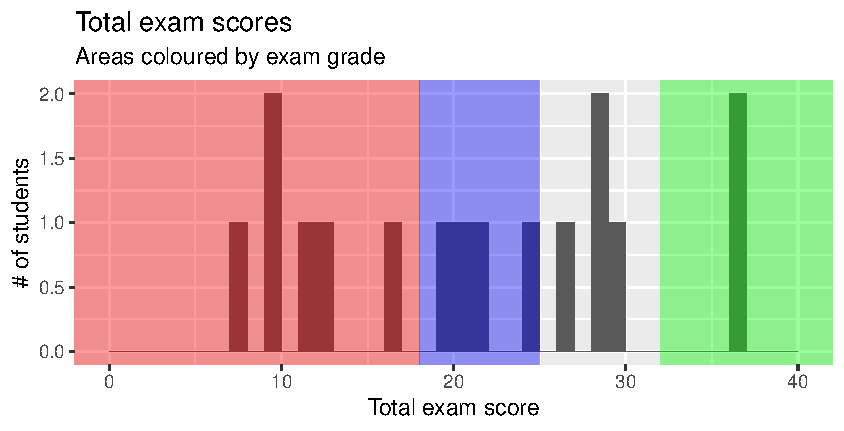
\includegraphics[width = 0.8\textwidth]{totalscore.pdf}
  \caption[Total score figure]{Plot of the total scores gotten by each student on the exam.}
  \label{fig:total_scores}
\end{figure}

The overall distribution of exam scores is illustrated in Figure \ref{fig:total_scores}. A total of sixteen students wrote the exam, of whom ten passed it. The mean and median score of all students was a touch over $21$,\sidenote[][]{Median $21.125$, mean $21.34$.} but as can be seen in the figure, and as is usual on most exams, there was a clear gap of a few students who failed with very low scores, with the rest passing -- only one student ended up just barely failing. The mean and median score among \emph{passing} students were $27.35$ and $27.375$ respectively.

\begin{figure}
  \centering
  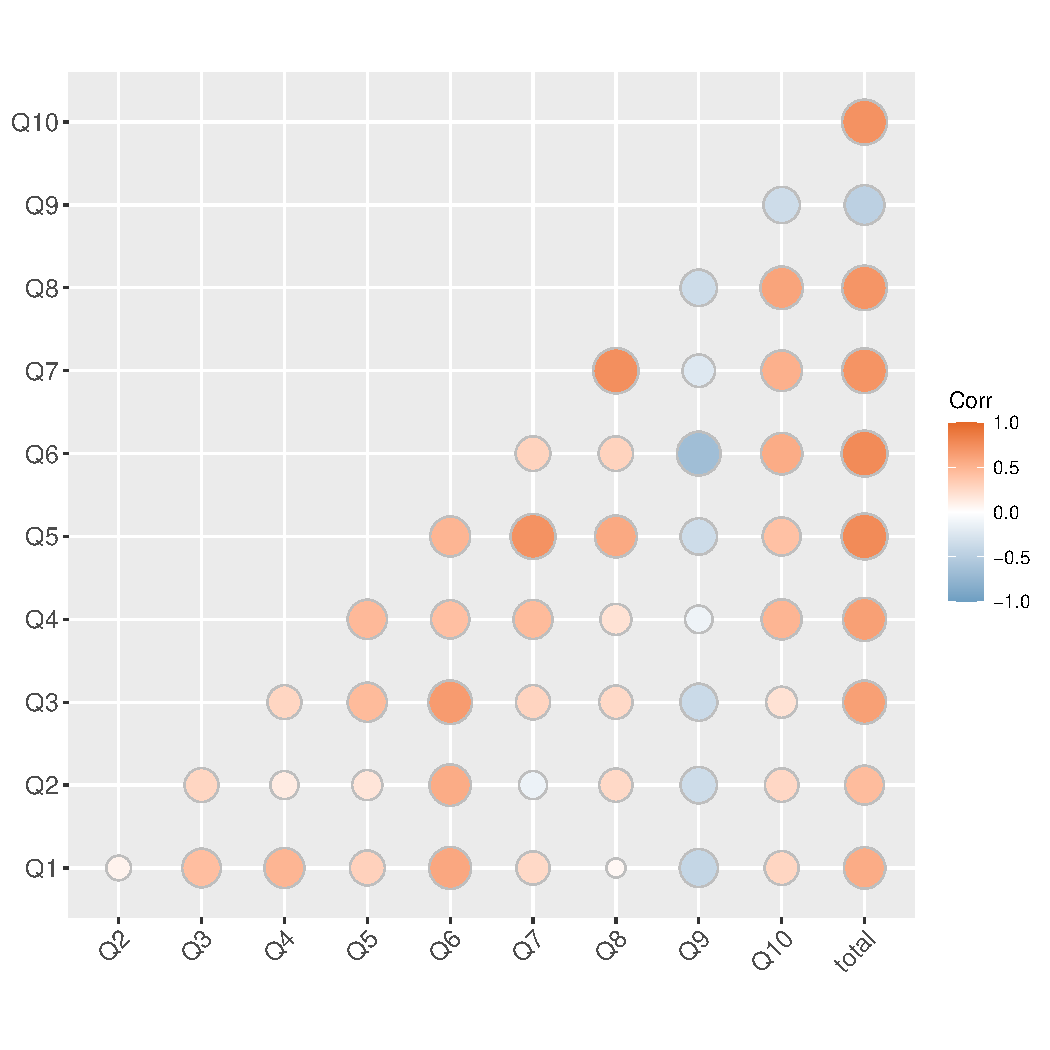
\includegraphics[width = 0.9\textwidth]{correlation_matrix.pdf}
  \caption[Score correlation matrix]{Correlation matrix for scores on each question, and on the exam as a whole.}
  \label{fig:corrplot}
\end{figure}

In Figure \ref{fig:corrplot}, one can see a correlation plot of correlations between scores on the different questions and with the total score. As expected, most questions correlate with each other -- doing well on one question tends to indicate that you understood the course well overall.

The one noticeable exception is question nine, which actually has a \emph{negative} correlation with the overall score. The reason for this is presumably that the question was hard, and each student only had to answer eight out of the ten questions. So the best-performing students chose this question as one of the two to not answer, and thus get a zero on. Why the lower-scoring students chose to answer this one might have two plausible explanations:
\begin{enumerate}
  \item They already had at least two of the other questions which they did not recall the answer for, and so they lost nothing by making an attempt at question nine and getting some score for it.
  \item Some may have misunderstood the question and not realized its difficulty, believing their incorrect solutions to actually be correct. Several students mistakenly believed that all directed acyclic graphs must be trees, and gave an answer that would have been roughly correct under that false assumption.
\end{enumerate}

\section{Question 1 (5p)} % about L10

\begin{quotation}
  What does it mean for a graph to be $k$-connected? State a correct definition.

  We proved a characterisation of two-connected graphs as being exactly the graphs that can be constructed by a certain process starting from a cycle graph. State the theorem, and give a proof of it.
\end{quotation}

This appears to have been a reasonable question, in that most students attempted it, and it got a wide range of scores.

\begin{figure}[p]
  \centering
  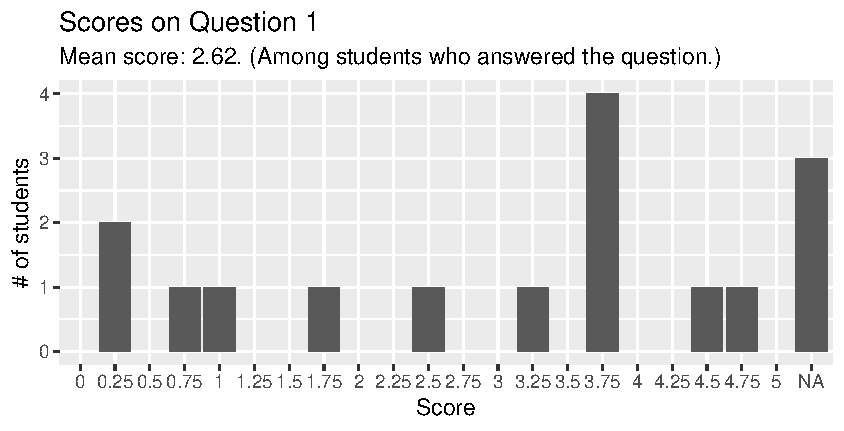
\includegraphics[width = \textwidth]{Q1.pdf}
  \caption[Score histogram for Q1]{Histogram of student scores on question one.}
  \label{fig:Q1}
\end{figure}

\section{Question 2 (5p)} % about L4

\begin{quotation}
  Define the adjacency matrix $A$, incidence matrix $D$, and Laplacian matrix $Q$ of a graph. Prove that $Q = DD^t$.
\end{quotation}

This question had the highest average score among the students who chose to answer it, so in some sense it was probably the easiest question on the exam -- perhaps together with question six, which had a nearly as high average, but got answered by every student writing the exam.

\begin{figure}[p]
  \centering
  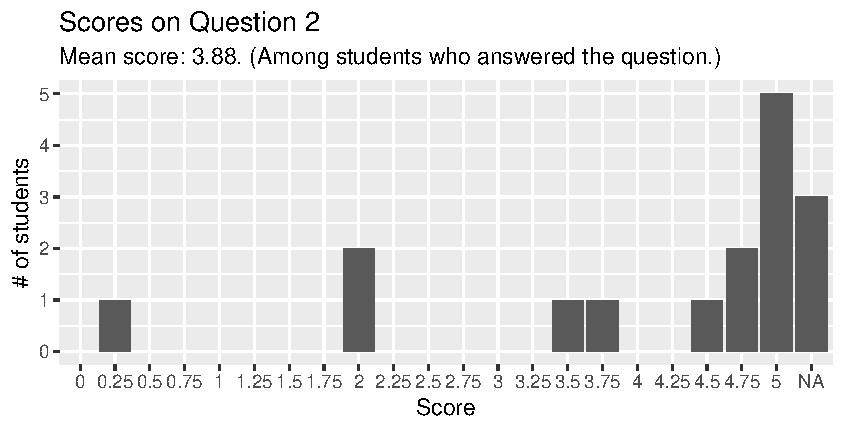
\includegraphics[width = \textwidth]{Q2.pdf}
  \caption[Score histogram for Q2]{Histogram of student scores on question two.}
  \label{fig:Q2}
\end{figure}

\section{Question 3 (5p)} % about L7

\begin{quotation}
  Recall that Hall's marriage theorem gives a condition for the existence of a matching of one side of a bipartite graph into the other in terms of a condition on the size of sets $Q \subseteq A$ and their neighbour sets $N(Q) \subseteq B$.

  Give a precise statement of the theorem, and then give a proof. (The proof we gave in the lecture was a clever application of the max-flow min-cut theorem, where we turned our bipartite graph into a flow network. If you choose to give this proof, please also draw a figure of the construction.)
\end{quotation}

Question three was seemingly among the harder questions, given the number of students who opted not to answer it. However, of those who answered it, everyone got at least one point, by correctly drawing the figure the question asks for.

\begin{figure}[p]
  \centering
  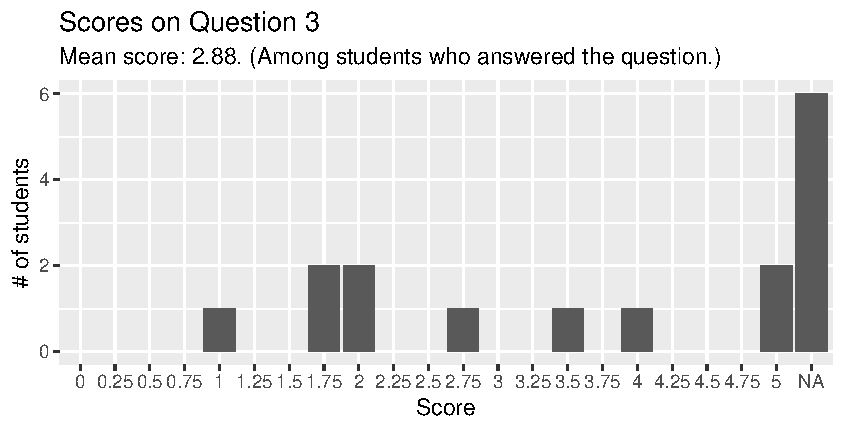
\includegraphics[width = \textwidth]{Q3.pdf}
  \caption[Score histogram for Q3]{Histogram of student scores on question three.}
  \label{fig:Q3}
\end{figure}

\section{Question 4 (5p)} % about L6
\begin{quotation}
  \textbf{Part a:} Prove that if you remove $k$ edges from a tree $T$, (Where the tree has more than $k$ vertices, so there are indeed $k$ edges to remove.) the resulting graph is a forest of $k+1$ trees.
  \vspace{0.5cm}

  \noindent
  \textbf{Part b:} Pick one of Kruskal's or Prim's algorithms. State it and prove its correctness.
\end{quotation}

This question, and question five and six, are the only questions for which every student submitted an answer -- which may be part of why the average score achieved on the question is comparatively low. On the other hand, questions five and six have comparatively high average scores.

Another explanation for why the scores are a bit low here may be that I was relatively strict on including all the details in my grading of the first part, because the statement of it is so simple.

\begin{figure}[p]
  \centering
  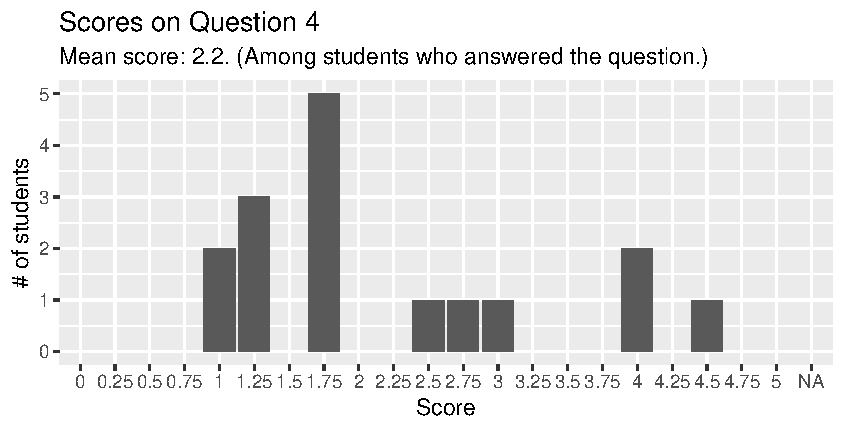
\includegraphics[width = \textwidth]{Q4.pdf}
  \caption[Score histogram for Q4]{Histogram of student scores on question four.}
  \label{fig:Q4}
\end{figure}

\section{Question 5 (5p)} % about L11

\begin{quotation}
  What does it mean for a graph to be planar? What is the planar dual of a planar graph? Give definitions, and include a correct figure illustrating the definition.

  Prove the following result from the course: (Hint: Consider a spanning tree of $G$ and its complement in $G^*$.)
  \begin{theorem}[Euler's formula]
    Let $G = (V,E)$ be a connected planar graph, and let $f$ be the number of faces for some planar embedding of $G$. Then
    $$\abs{V} - \abs{E} + f = 2,$$
    and so in particular any two planar embeddings have the same number of faces.
  \end{theorem}
\end{quotation}

Every student chose to answer this question, presumably because every student did recall the definition of being planar, and most could also correctly or nearly-correctly\sidenote[][]{Many forgot that the planar dual is a multigraph.} define the planar dual. The average on this question is thus fairly high.

\begin{figure}[p]
  \centering
  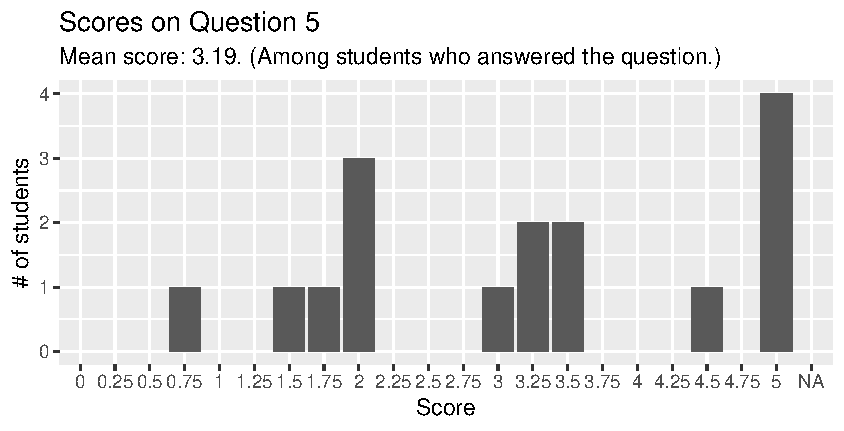
\includegraphics[width = \textwidth]{Q5.pdf}
  \caption[Score histogram for Q5]{Histogram of student scores on question five.}
  \label{fig:Q5}
\end{figure}

\section{Question 6 (5p)} % about L2

\begin{quotation}
  What does it mean for a graph to be Eulerian? State and prove Euler's theorem giving a criterion for a graph to be Eulerian.
\end{quotation}

This question got a rather high average, and was answered by every student writing the exam -- so together with question two, this was probably the easiest question on the exam.

\begin{figure}[p]
  \centering
  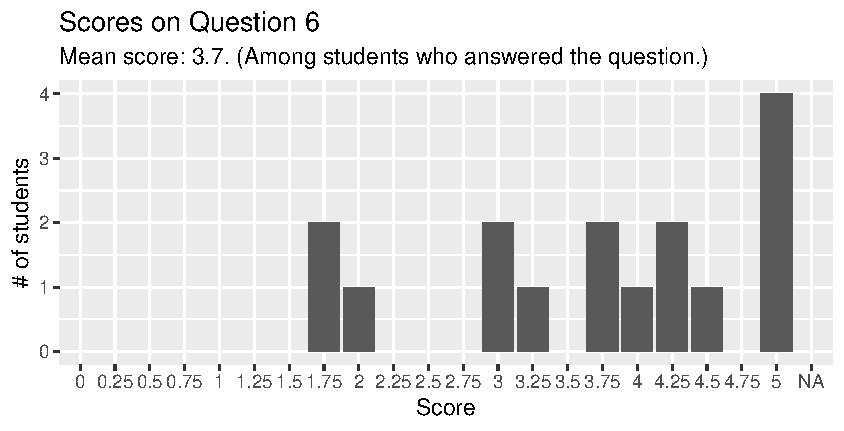
\includegraphics[width = \textwidth]{Q6.pdf}
  \caption[Score histogram for Q6]{Histogram of student scores on question six.}
  \label{fig:Q6}
\end{figure}

\section{Question 7 (5p)} % about L14

\begin{quotation}
  Recall from the lectures that the \emph{minimum bisection problem} asks for a partition of the vertices of a graph into two equally-sized sets (So, as we state it, it only applies to graphs with an even number of vertices.) such that the number of edges between them is minimal.

  We proved an upper bound on how many edges you could be forced to include in such a bisection using the probabilistic method, where we started by picking a matching on the complement graph. State and prove this result.
\end{quotation}

This question was evidently seen as hard by the students, since ten out of sixteen students opted not to answer this question. It may be because this particular result was not so prominent among the things we proved using the probabilistic method, and so people simply did not remember it -- or it could be that the probabilistic method in general is seen as hard. That was certainly the case in the Combinatorics course, though it is of course hard to compare things between courses.

\begin{figure}[p]
  \centering
  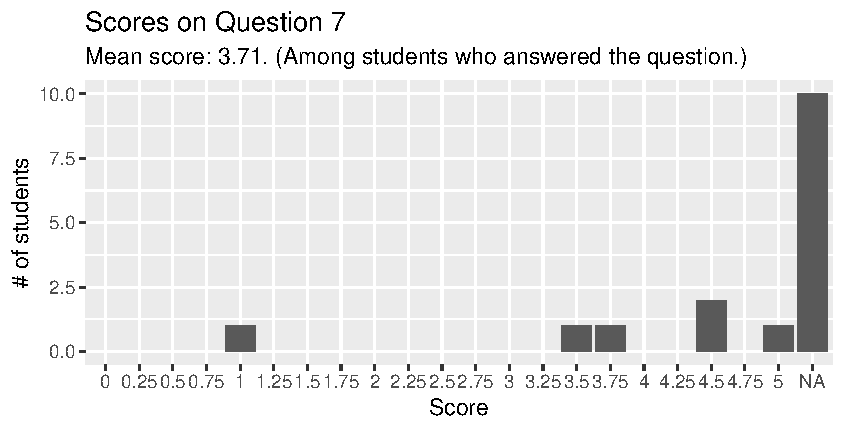
\includegraphics[width = \textwidth]{Q7.pdf}
  \caption[Score histogram for Q7]{Histogram of student scores on question seven.}
  \label{fig:Q7}
\end{figure}

\section{Question 8 (5p)} % about L18

\begin{quotation}
  Given a graph $H$ and an integer $n$, define the extremal function $\ex(n; H)$ of $H$.

  Turáns theorem says that
  $$\ex(n; K_{r+1}) \leq \left(1 - \frac{1}{r}\right)\frac{n^2}{2}.$$
  Prove this. (We gave two proofs in the course, and there are many more pretty proofs floating around. Any correct proof is of course a correct answer to the question. The first proof we gave in the course used the Caro-Wei result on independent sets, and then applied the Cauchy-Schwarz inequality
  $$\abs{\langle a, b \rangle} \leq \norm{a}\norm{b}$$
  to a clever choice of $a$ and $b$.)
\end{quotation}

Just like question seven, ten out of sixteen students skipped this question entirely, and the average score of those who tried is not too different. Perhaps the difficulty of this question stems from needing to remember what the Caro-Wei result said, and how to apply it to this question? Every student who did respond attempted that proof strategy, though we did also do an alternative proof of the same result in class.

\begin{figure}[p]
  \centering
  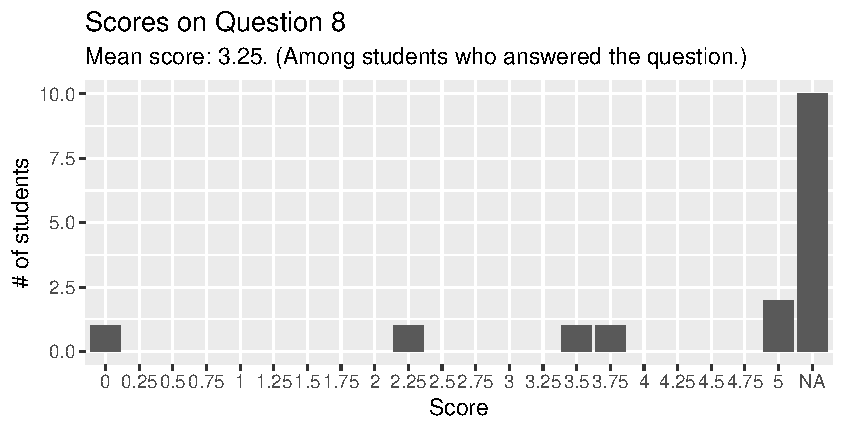
\includegraphics[width = \textwidth]{Q8.pdf}
  \caption[Score histogram for Q8]{Histogram of student scores on question eight.}
  \label{fig:Q8}
\end{figure}

\section{Question 9 (5p)} % surprise stuff!

\begin{quotation}
  A \emph{directed acyclic graph} (often called just a \emph{DAG}) is a directed graph that contains no cycles. Devise a reasonable (That is, not just a brute-force method, but something you'd actually use in practice.) algorithm for determining when such a graph is Hamiltonian. For directed graphs, being Hamiltonian means having a \emph{directed} Hamiltonian path.
\end{quotation}

This question was by far the hardest question on the exam, and nine students recognized it as such and did not answer. Of the remaining students, not a single one gave an algorithm that would actually work -- so the abysmal average score in fact hides a somewhat lenient grading, where one could get up to $2.5$ points for an incorrect solution that had at least some rationale for why it might work.\sidenote[][]{The student who got $2.5$ mistakently believed that all DAGs are trees, but then gave a correct algorithm for determining if a tree has a Hamiltonian path.}

\begin{figure}[p]
  \centering
  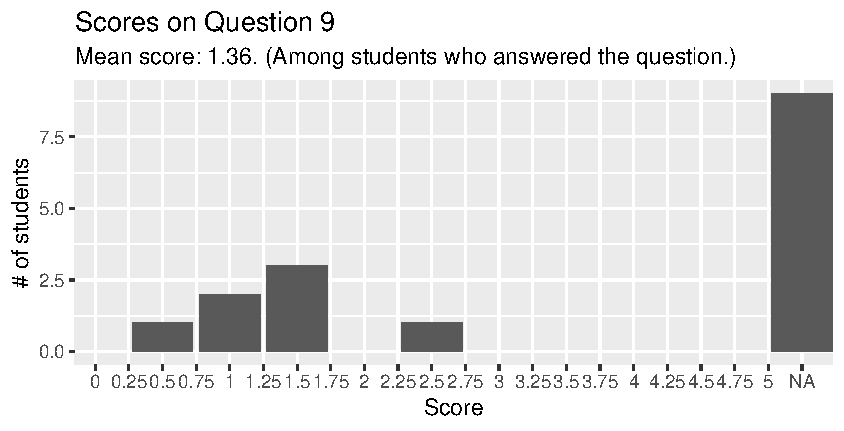
\includegraphics[width = \textwidth]{Q9.pdf}
  \caption[Score histogram for Q9]{Histogram of student scores on question nine.}
  \label{fig:Q9}
\end{figure}

\section{Question 10 (5p)} % surprise stuff!

\begin{quotation}
  For each of these statements, determine if it is true or false and give a proof or disproof:
  \begin{enumerate}[label=\alph*)]
    \item For every $k\geq 3$, there exists a $k$-regular Hamiltonian graph.
    \item For every $k \geq 1$, there exists a $k$-regular planar graph.
    \item For every $k \geq 1$, there exists a multigraph with exactly $k$ spanning trees.
    \item For every $k \geq 1$, there exists a graph with exactly $k$ spanning trees.
    \item There exists a $6$-connected planar graph.
    \item There exists a tree in which every vertex has degree $2$.
  \end{enumerate}
\end{quotation}

\begin{figure}[p]
The results on this question are interesting, as most students tried it, and it displays the greatest spread of results. Presumably this is because most students were able to do at least one or two of the statements. 

Performance on this question is probably the best predictor of overall performance on the exam -- if I had graded the entire exam solely based off of ``did you get at least $2.25$ points on question 10'', thirteen out of sixteen students would have gotten a correct assignment to pass or fail, and a corresponding scheme for assigning letter grades would get ten out of sixteen students right.

  \centering
  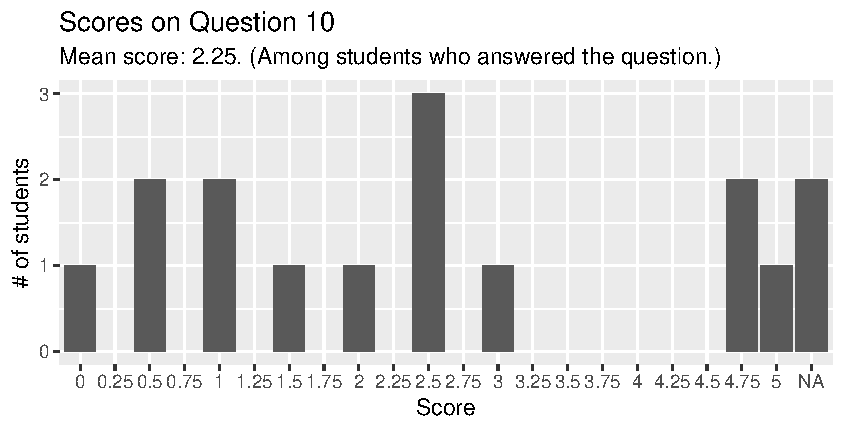
\includegraphics[width = \textwidth]{Q10.pdf}
  \caption[Score histogram for Q10]{Histogram of student scores on question ten.}
  \label{fig:Q10}
\end{figure}

\end{document}
